\documentclass[a4paper]{arrowhead}

\usepackage[yyyymmdd]{datetime}
\usepackage{etoolbox}
\usepackage[utf8]{inputenc}
\usepackage{multirow}
\usepackage{hyperref}

\renewcommand{\dateseparator}{-}

\setlength{\parskip}{1em}

%% Special references
\newcommand{\fref}[1]{{\textcolor{ArrowheadBlue}{\hyperref[sec:functions:#1]{#1}}}}
\newcommand{\mref}[1]{{\textcolor{ArrowheadPurple}{\hyperref[sec:model:#1]{#1}}}}
\newcommand{\pdef}[1]{{\textcolor{ArrowheadGrey}{#1\label{sec:model:primitives:#1}\label{sec:model:primitives:#1s}\label{sec:model:primitives:#1es}}}}
\newcommand{\pref}[1]{{\textcolor{ArrowheadGrey}{\hyperref[sec:model:primitives:#1]{#1}}}}

\newrobustcmd\fsubsection[3]{
  \addtocounter{subsection}{1}
  \addcontentsline{toc}{subsection}{\protect\numberline{\thesubsection}function \textcolor{ArrowheadBlue}{#1}}
  \renewcommand*{\do}[1]{\rref{##1},\ }
  \subsection*{
    \thesubsection\quad
    operation
    \textcolor{ArrowheadBlue}{#1}
    (\notblank{#2}{\mref{#2}}{})
    \notblank{#3}{: \mref{#3}}{}
  }
  \label{sec:functions:#1}
}
\newrobustcmd\msubsection[2]{
  \addtocounter{subsection}{1}
  \addcontentsline{toc}{subsection}{\protect\numberline{\thesubsection}#1 \textcolor{ArrowheadPurple}{#2}}
  \subsection*{\thesubsection\quad#1 \textcolor{ArrowheadPurple}{#2}}
  \label{sec:model:#2} \label{sec:model:#2s} \label{sec:model:#2es}
}

\begin{document}

%% Arrowhead Document Properties
\ArrowheadTitle{Authentication Core System}
\ArrowheadType{System Description}
\ArrowheadTypeShort{SysD}
\ArrowheadVersion{5.0.0}
\ArrowheadDate{\today}
\ArrowheadAuthor{Tamás Bordi}
\ArrowheadStatus{DRAFT}
\ArrowheadContact{tbordi@aitia.ai}
\ArrowheadFooter{\href{www.arrowhead.eu}{www.arrowhead.eu}}
\ArrowheadSetup
%%

%% Front Page
\begin{center}
  \vspace*{1cm}
  \huge{\arrowtitle}

  \vspace*{0.2cm}
  \LARGE{\arrowtype}
  \vspace*{1cm}

  %\Large{Service ID: \textit{"\arrowid"}}
  \vspace*{\fill}

  % Front Page Image
  %\includegraphics{figures/TODO}

  \vspace*{1cm}
  \vspace*{\fill}

  % Front Page Abstract
  \begin{abstract}
    This document provides system description for the \textbf{Authentication Core System}.
  \end{abstract}

  \vspace*{1cm}

 \end{center}

\newpage
%%

%% Table of Contents
\tableofcontents
\newpage
%%

\section{Overview}
\label{sec:overview}
\color{black}
This document describes the Authentication core system, which exists to provide, manage and validate system identities within an Eclipse Arrowhead Local Cloud (LC).

The rest of this document is organized as follows.
In Section \ref{sec:prior_art}, we reference major prior art capabilities
of the system.
In Section \ref{sec:use}, we describe the intended usage of the system.
In Section \ref{sec:properties}, we describe fundamental properties
provided by the system.
In Section \ref{sec:delimitations}, we describe delimitations of capabilities
of the system.
In Section \ref{sec:services}, we describe the abstract services produced by the system.
In Section \ref{sec:security}, we describe the security capabilities
of the system.

\subsection{Significant Prior Art}
\label{sec:prior_art}

The strong development on cloud technology and various requirements for digitisation and automation has led to the concept of Local Clouds (LC).

\textit{"The concept takes the view that specific geographically local automation tasks should be encapsulated and protected."} \cite{jerker2017localclouds}

One of the main building blocks when realizing such Local Cloud is the capability of authenticating all the systems when wanted to join to a given LC and verifying the system identities before enabling service sessions between them. 

The previous versions of Arrowhead had no separated or outsourced authentication mechanisms, this task relied entirely on X.509 certificates. While it is working well and reliably, it might be too resource intensive for edge devices or it could be exaggerated for certain use cases. In order to fulfill the needs for various authentication mechanisms, Arrowhead 5.0 is introducing the Authentication Core System which enables to implement and deploy the preferred methods and utilize them in a standard manner.

\subsection{How This System Is Meant to Be Used}
\label{sec:use}

The Authentication is a recommended core system of Eclipse Arrowhead LC and is responsible for the fundamental system identity control functionality by storing system related data in order to being able to verify the provided credentials and assign identity tokens to the systems. Also, this core system has the responsibility to verify the identity tokens upon requests. 

IMPORTANT! Application systems should not share their identity tokens with other systems than the arrowhead core or support systems. For authenticated communication between application systems the authorization token should be used. A typical way of working from a consumer system perspective is described n Figure \ref{fig:auth_interactions}

\begin{itemize}
    \item The Figure describes a use case with a dynamic orchestration from the view of the consumer.
    \item Besides the consumer, every interaction with the core systems from the provider side and even the internal communication between the core systems requires identity tokens, but these are omitted here for the sake of easier understanding.
    \item Interactions between the consumer and provider does not contain identity token in order to prevent any kind of identity theft. Identities should be only shared with the trusted core and support systems.
    \item The difference between the identity and authorization tokens is that while identity tokens identify a system only, the authentication tokens are representing a consumer-provider service (optionally operation) exchange session.
    \item Having an identity token is a must for all the systems, but requiring an authorization token is a matter of choice of the provider systems.
\end{itemize}

\begin{figure}[ht!]
  \centering
  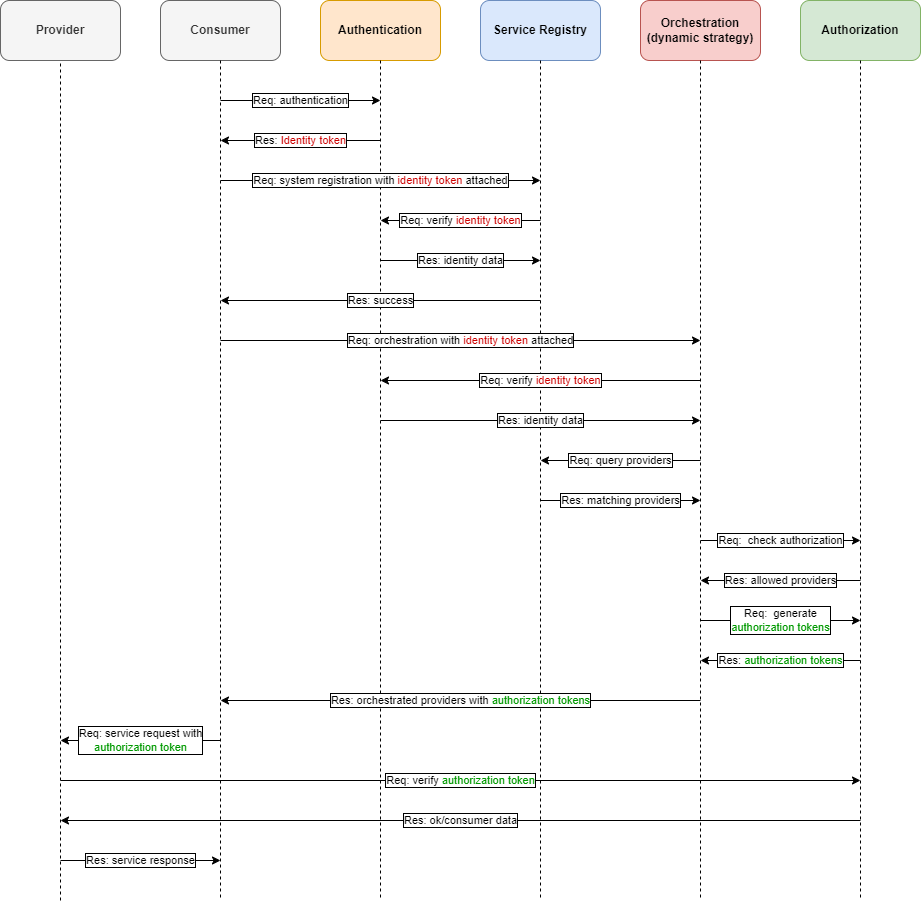
\includegraphics[width=\textwidth]{figures/auth_interactions}
  \caption{Interaction diagram of a typical use case. }
  \label{fig:auth_interactions}
\end{figure}

\newpage

\subsection{System functionalities and properties}
\label{sec:properties}

\subsubsection {Functional properties of the system}

Authentication solves the following needs to fulfill the requirements of authentication and system identity management.

\begin{itemize}
    \item Enables the core, support and application systems to login/logout into/from the LC.
    \item Enables the core/support systems to validate that an other system is authenticated and already part of the LC.
    \item Enables the core/support systems to gather identity related data about a requesting system.
    \item Enabled the core/support systems with management rights to add, query and revoke system credentials.
    \item Enabled the core/support systems with management rights to query and close active login sessions.
    \item Enables the cloud operators to implement different kind of authentication methods.
\end{itemize}

\subsubsection {Non functional properties of the system}
-

\subsubsection {Data stored by the system}
In order to achieve the mentioned functionalities, Authentication is capable to store the following information set:

\begin{itemize}
    \item \textbf{System authentication method}: What type of authentication method is assigned to a system by system name.
    \item \textbf{System authentication info}: What is required to verify upon a login request by system name and whether the system has access rights to the management services by default or not.
    \item \textbf{Identity tokens}: the assigned identity tokens by system-name and with the token properties like start date, expiration date, etc... .
\end{itemize}

\subsection{Important Delimitations}
\label{sec:delimitations}

-

\newpage

\section{Services produced}
\label{sec:services}

\msubsection{service}{identity}
The purpose of this service is to enable the core/support and application systems to login/logout into/out from the Local Cloud and also to enable core/support systems to verify a requester application system's identity.

\msubsection{service}{identity-management}
Its main purpose is to manage the system credentials and the active sessions in bulk. It also provides querying functionalities. The service is offered for core and administrative support systems.

\msubsection{service}{monitor}
Recommended service. Its purpose is to give information about the Authentication system itself. The service is offered for both application and core/support systems.

\newpage

\section{Security}
\label{sec:security}

The actual implementation of the Authentication Core System can decide about the encryption of the connection between itself and other systems.
 
\newpage

\bibliographystyle{IEEEtran}
\bibliography{bibliography}

\newpage

\section{Revision History}
\subsection{Amendments}

\noindent\begin{tabularx}{\textwidth}{| p{1cm} | p{3cm} | p{2cm} | X | p{4cm} |} \hline
\rowcolor{gray!33} No. & Date & Version & Subject of Amendments & Author \\ \hline

1 & YYYY-MM-DD & \arrowversion & & Xxx Yyy \\ \hline
\end{tabularx}

\subsection{Quality Assurance}

\noindent\begin{tabularx}{\textwidth}{| p{1cm} | p{3cm} | p{2cm} | X |} \hline
\rowcolor{gray!33} No. & Date & Version & Approved by \\ \hline

1 & YYYY-MM-DD & \arrowversion  &  \\ \hline

\end{tabularx}

\end{document}